	\documentclass{beamer}
	\usepackage[utf8]{inputenc}
	\usepackage{graphicx}
	\usepackage{booktabs}
	\usepackage{caption}
	\usetheme{Madrid}
	\usepackage{graphicx}
	\usepackage{hyperref}
	\usepackage{listings}
	\usepackage{xcolor}
	\usepackage{multirow}

	
	\title{PairCoder: A Multi-Agent Framework for Code Generation}
	\author{Taylan Bapur, Jan H\"artrich}
	\date{Summer 2025 -- Seminar on Machine Learning in Software Engineering}
	
	\definecolor{codegray}{rgb}{0.5,0.5,0.5}
	\lstdefinestyle{mystyle}{
	    backgroundcolor=\color{white},
	    commentstyle=\color{gray},
	    keywordstyle=\color{blue},
	    numberstyle=\tiny\color{codegray},
	    stringstyle=\color{red},
	    basicstyle=\ttfamily\footnotesize,
	    breakatwhitespace=false,
	    breaklines=true,
	    captionpos=b,
	    keepspaces=true,
	    numbers=left,
	    numbersep=5pt,
	    showspaces=false,
	    showstringspaces=false,
	    showtabs=false,
	    tabsize=2
	}
	\lstset{style=mystyle}
	
	
	\begin{document}
	
	\begin{frame}
	  \titlepage
	\end{frame}
	
	\begin{frame}{Agenda}
	  \tableofcontents
	\end{frame}
	
	\section{Introduction}
	\begin{frame}{Motivation}
	  \begin{itemize}
	    \item LLMs are effective at code completion and simple programming tasks.
	    \item Struggle with complex logic, dependencies, and iterative problem-solving.
	    \item Multi-agent frameworks offer collaboration, adaptability, and robustness.
	  \end{itemize}
	\end{frame}
	
	\begin{frame}{Overview of Frameworks}
	  \begin{itemize}
	    \item \textbf{PairCoder}: Navigator and Driver collaborate iteratively.
	    \item \textbf{Guided Code Generation}: Decomposes tasks hierarchically.
	    \item \textbf{MapCoder}: Simulates full development cycle with 4 agents.
	  \end{itemize}
	\end{frame}
	
	\section{PairCoder}
	\begin{frame}{PairCoder Architecture}
	  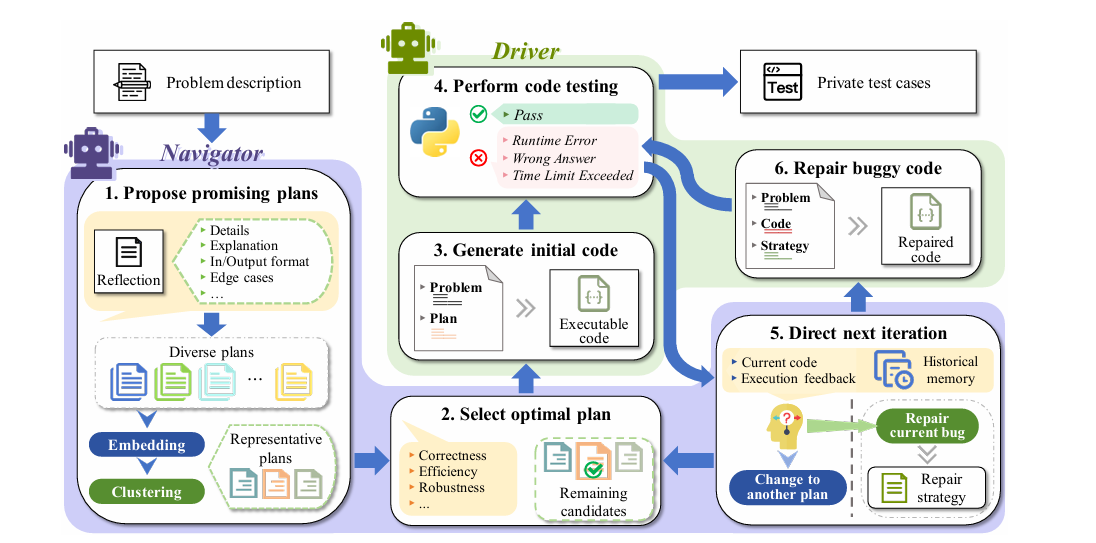
\includegraphics[width=0.85\textwidth]{paircoder-architecture.png}
	  \begin{itemize}
	    \item Navigator plans, Driver implements and tests.
	    \item Iterative loop mimics human pair programming.
	  \end{itemize}
	\end{frame}
	
	\begin{frame}{Navigator Role}
	  \begin{itemize}
	    \item Reflects on problem and generates multiple solution plans.
	    \item Uses clustering to pick diverse, promising strategies.
	    \item Analyzes feedback to refine or switch plans.
	  \end{itemize}
	\end{frame}
	
	\begin{frame}{Driver Role}
	  \begin{itemize}
	    \item Implements code from selected plan.
	    \item Runs public test cases.
	    \item Applies Navigator's suggested fixes.
	  \end{itemize}
	\end{frame}
	
	\begin{frame}{Iterative Workflow}
	  \begin{enumerate}
	    \item Navigator proposes a plan.
	    \item Driver generates code.
	    \item Code is tested and classified.
	    \item Navigator reacts to feedback.
	  \end{enumerate}
	\end{frame}
	
	\begin{frame}{Example Problem}
	  \begin{itemize}
	    \item Task: Ensure $a[i] \leq i+1$ by inserting elements.
	    \item Initial code fails for some edge cases.
	    \item Navigator detects logic flaw.
	  \end{itemize}
	\end{frame}
	

	
	
	
	\begin{frame}[fragile]{Buggy Code (Fails Tests)}
	\scriptsize
	\begin{verbatim}
	def solve_buggy(arr):
	    operations = 0
	    for i in range(len(arr)):
	        if arr[i] > i + 1 and arr[i+1] < arr[i]:
	            operations += 1
	    return operations
	\end{verbatim}
	\end{frame}
	
	\begin{frame}[fragile]{Fixed Code (Passes Tests)}
	\scriptsize
	\begin{verbatim}
	def solve_fixed(arr):
	    arr = arr[:]
	    i = 0
	    ops = 0
	    while i < len(arr):
	        if arr[i] > i + 1:
	            arr.insert(i, i + 1)
	            ops += 1
	        else:
	            i += 1
	    return ops
	\end{verbatim}
	\end{frame}
	

	\begin{frame}{Demo Tooling}
	  \begin{itemize}
	    \item Live Demo
	  \end{itemize}
	\end{frame}



	\begin{frame}{Key Techniques}
	  \begin{itemize}
	    \item Multi-plan exploration using clustering.
	    \item Feedback-driven refinement loop.
	    \item State tracking to avoid repetition.
	  \end{itemize}
	\end{frame}
	
	\begin{frame}{Evaluation Results}
	  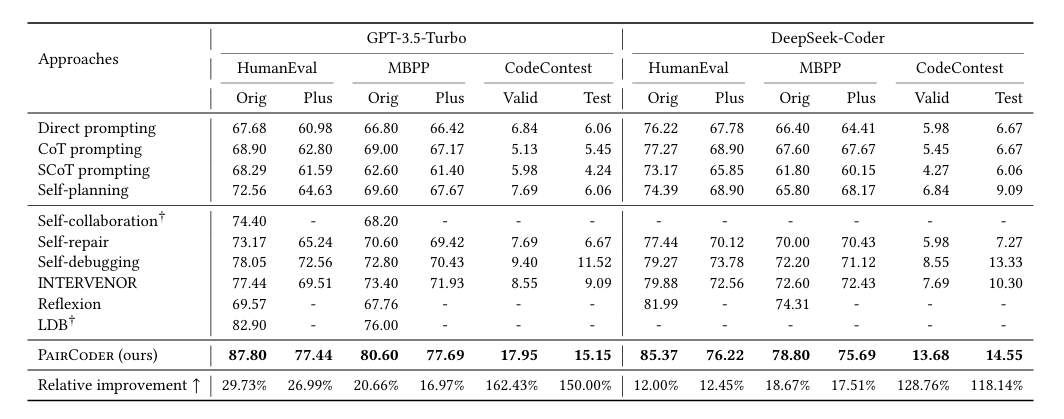
\includegraphics[width=0.85\textwidth]{paircoder-results.png}
	  \begin{itemize}
	    \item Up to 87.8\% on HumanEval.
	    \item Outperforms CoT, Self-debugging.
	    \item Gains most from refinement loop.
	  \end{itemize}
	\end{frame}
	
	\begin{frame}{What did we get?}
	  \begin{table}
	    \centering
	    \begin{tabular}{l l r r}
	      \toprule
	      \textbf{Benchmark} & \textbf{Split} & \textbf{Score (\%)} & \textbf{Overall (\%)} \\
	      \midrule
	      mbpp        & test  & 76.74 & \multirow{2}{*}{79.37} \\
	      mbpp        & plus  & 85.00 & \\
	      \midrule
	      humaneval   & raw   & 90.00 & \multirow{2}{*}{67.50} \\
	      humaneval   & plus  & 45.00 & \\
	      \midrule
	      codecontest & test  &  0.00 & \multirow{2}{*}{27.78} \\
	      codecontest & valid & 38.46 & \\
	      \bottomrule
	    \end{tabular}
	  \end{table}
	   \begin{itemize}
	    \item mbpp 63 tests
	    \item humaneval 40 tests
	    \item codecontest 18 tests
	    \item https://github.com/ELSATOAH/A-Pair-Coder
	  \end{itemize}
	\end{frame}



	
	\section{Guided Code Generation}
	\begin{frame}{Guided Code Gen Overview}
	  \begin{itemize}
	    \item Generalist Agent decomposes problem.
	    \item Code Agents solve atomic tasks.
	    \item Tester Agent validates components.
	  \end{itemize}
	\end{frame}
	
	\begin{frame}{Comparison with PairCoder}
	  \begin{itemize}
	    \item Guided Code is modular and hierarchical.
	    \item PairCoder is iterative and flexible.
	    \item Trade-off: structure vs. adaptability.
	  \end{itemize}
	\end{frame}
	
	\section{MapCoder}
	\begin{frame}{MapCoder Overview}
	  \begin{itemize}
	    \item Simulates full development cycle.
	    \item 4 agents: Retrieval, Planning, Coding, Debugging.
	    \item Inspired by human-like software pipelines.
	  \end{itemize}
	\end{frame}
	
	\begin{frame}{MapCoder Architecture}
	  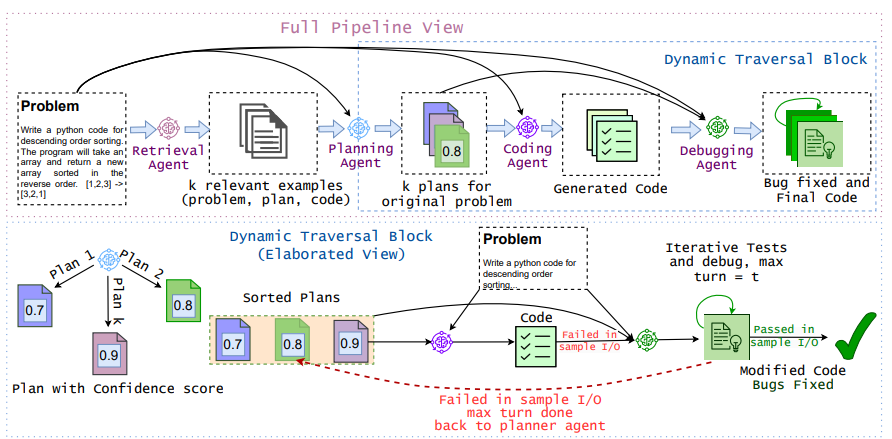
\includegraphics[width=0.85\textwidth]{mapcoder-architecture.png}
	  \begin{itemize}
	    \item Pipeline with dynamic traversal.
	    \item Switches plans on failure.
	  \end{itemize}
	\end{frame}
	
	\begin{frame}{Agent Roles in MapCoder}
	  \begin{itemize}
	    \item Retrieval Agent: Fabricates examples.
	    \item Planning Agent: Generates multiple plans + scores.
	    \item Coding Agent: Implements plan.
	    \item Debugging Agent: Refines code iteratively.
	  \end{itemize}
	\end{frame}
	
	\begin{frame}{MapCoder Evaluation}
	  \begin{itemize}
	    \item 93.9\% pass@1 on HumanEval.
	    \item SOTA results across benchmarks.
	    \item Best suited for hard problems.
	  \end{itemize}
	\end{frame}
	
	\section{Comparison and Conclusion}
	\begin{frame}{Framework Comparison}
	  \begin{itemize}
	    \item \textbf{PairCoder:} Agile, mid-sized tasks.
	    \item \textbf{Guided Code:} Best for structured problems.
	    \item \textbf{MapCoder:} Full pipeline, highest accuracy.
	  \end{itemize}
	\end{frame}
	
	\begin{frame}{Conclusion}
	  \begin{itemize}
	    \item Multi-agent systems improve LLM coding.
	    \item Each method has strengths.
	    \item Hybrid approaches are promising.
	    \item Tool reproducibility is a challenge.
	  \end{itemize}
	\end{frame}
	
	\begin{frame}
	  \centering
	  \Huge Questions?
	\end{frame}
	
	\end{document}
